\section{Digital Receiver Hardware}

The digital receiver has been designed to interface with the hardware used in the original analog polarimeter. As such, very few modifications are required to the original front end.

The new design does however require down-conversion of the signal into the 0$\rightarrow$1000~MHz band suitable for ADC sampling. This requires the design and construction of downmixers and suitable band defining filters before the input to the ADC's.

\subsection{Down mixer}
\label{sec:mixers}
Hittite manufactures the HMC129LC4 MMIC which is suitable for our purposes. We used Ansoft Designer to simulate a design based around using the HMC129LC4. This design was then manufactured and packaged in house, and compared successfully with test boards sent by Hittite (see Appendix~\ref{sec:mixerResults}).

\begin{figure}
 \centering
 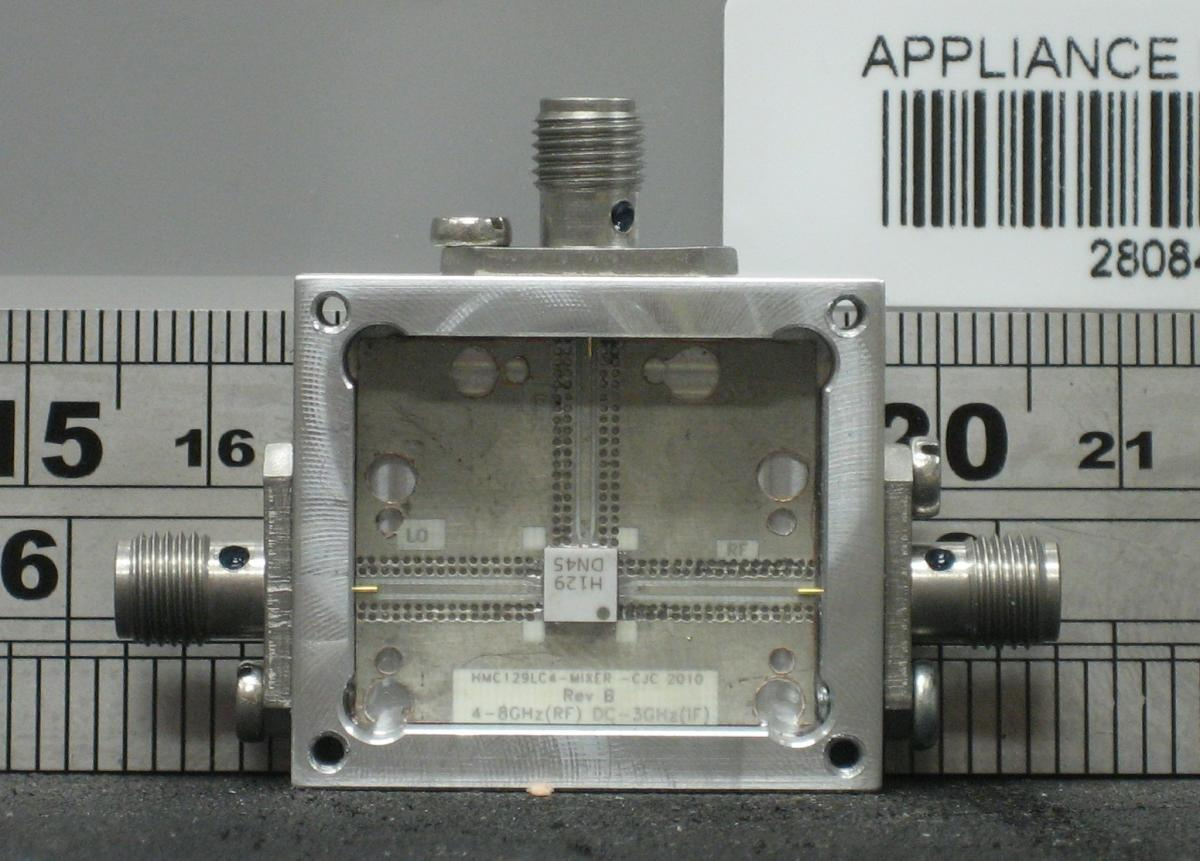
\includegraphics[width=0.5\textwidth]{./images/mixers/mixera.jpg}
 % mixer.jpg: 1551x1113 pixel, 72dpi, 54.72x39.26 cm, bb=
 \caption{The HMC129LC4 prototype mixer. The substrate is  RO4350 250$\mu$m duroid ($\epsilon=3.66$) with $\frac{1}{2}$~oz/ft$^{2}$ Copper layer (17.5$\mu$m). }
 \label{fig:mixer}
\end{figure}

\subsubsection{Mixer Results}
\label{sec:mixerResults}
\begin{figure}[ht]
 \centering
\subfloat[RF Return Loss(Magnitude)]{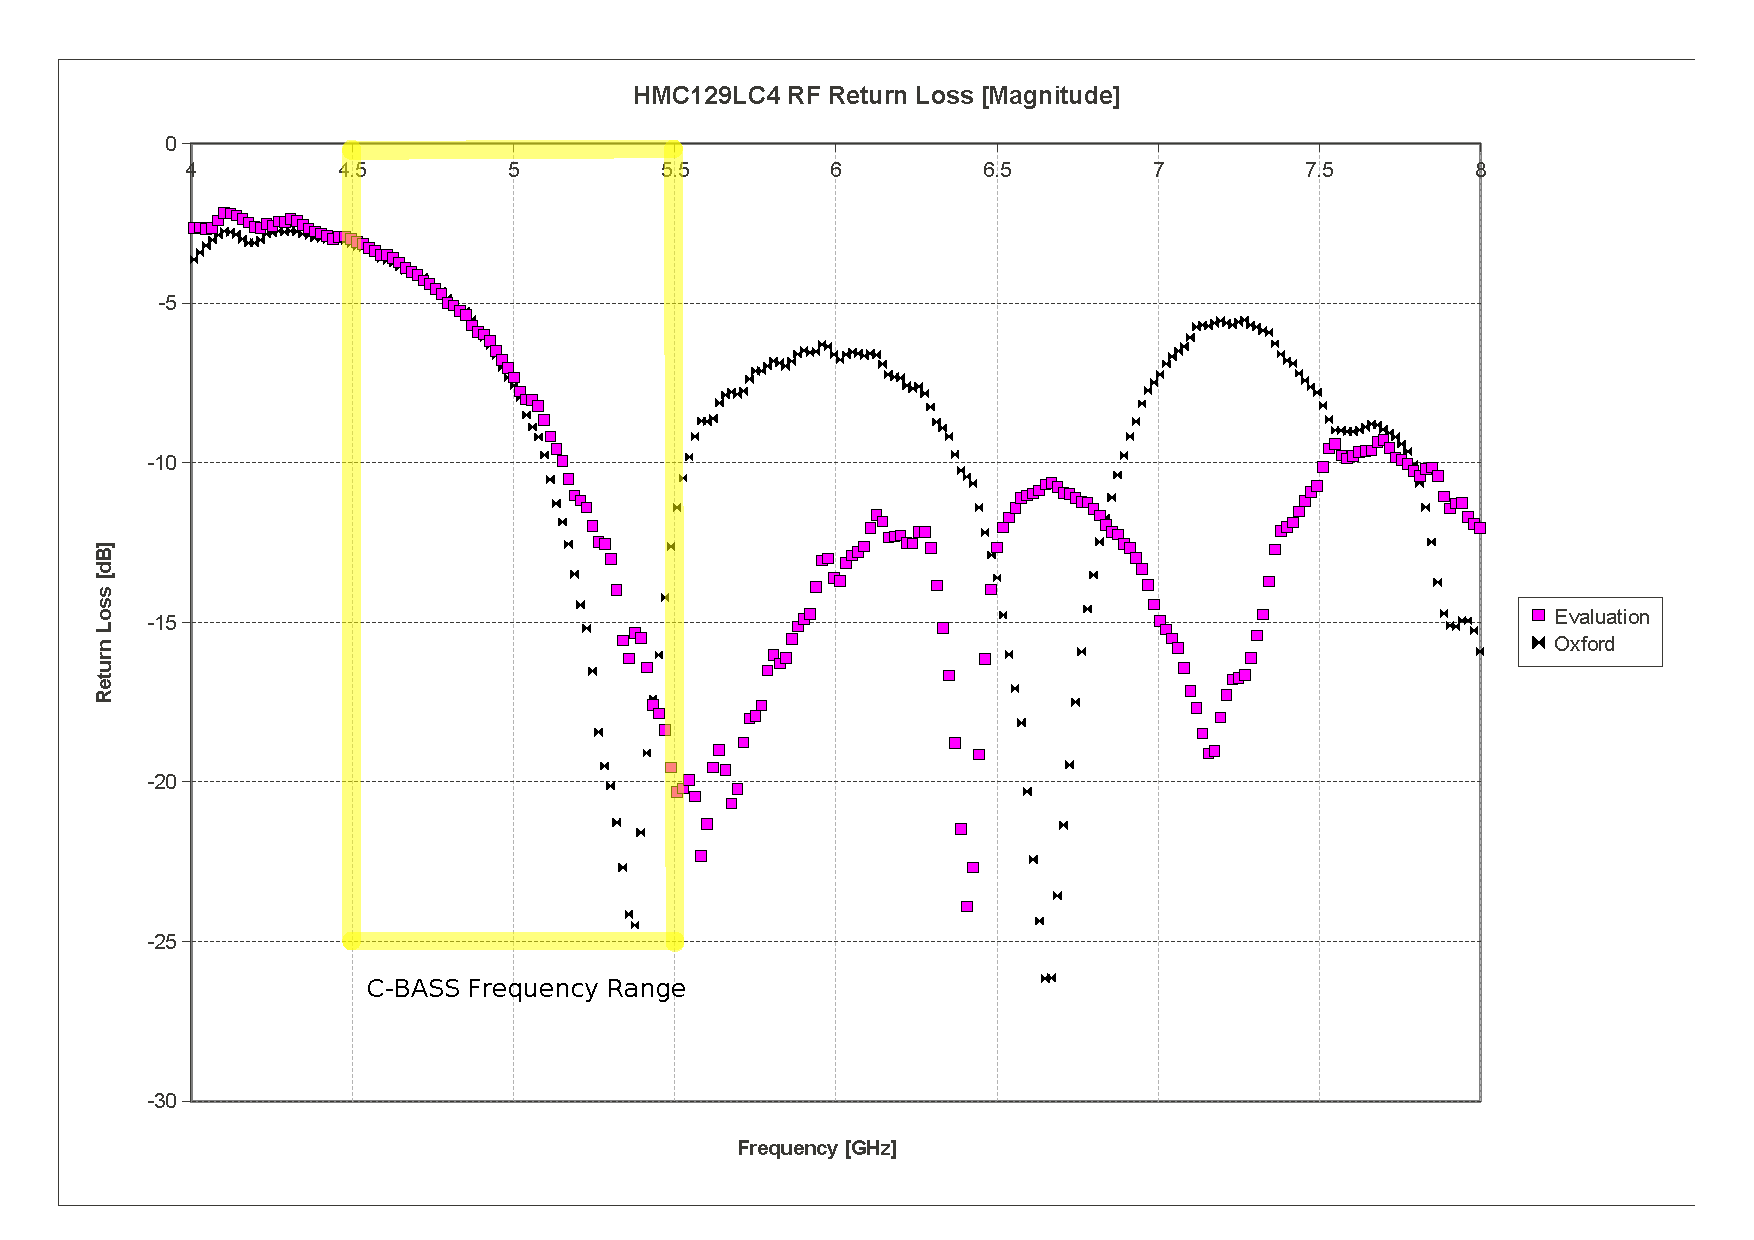
\includegraphics[width=\textwidth]{images/mixers/pg_0001a.pdf}}
\hspace{0.1cm}
%\subfloat[RF Return Loss(Phase)]{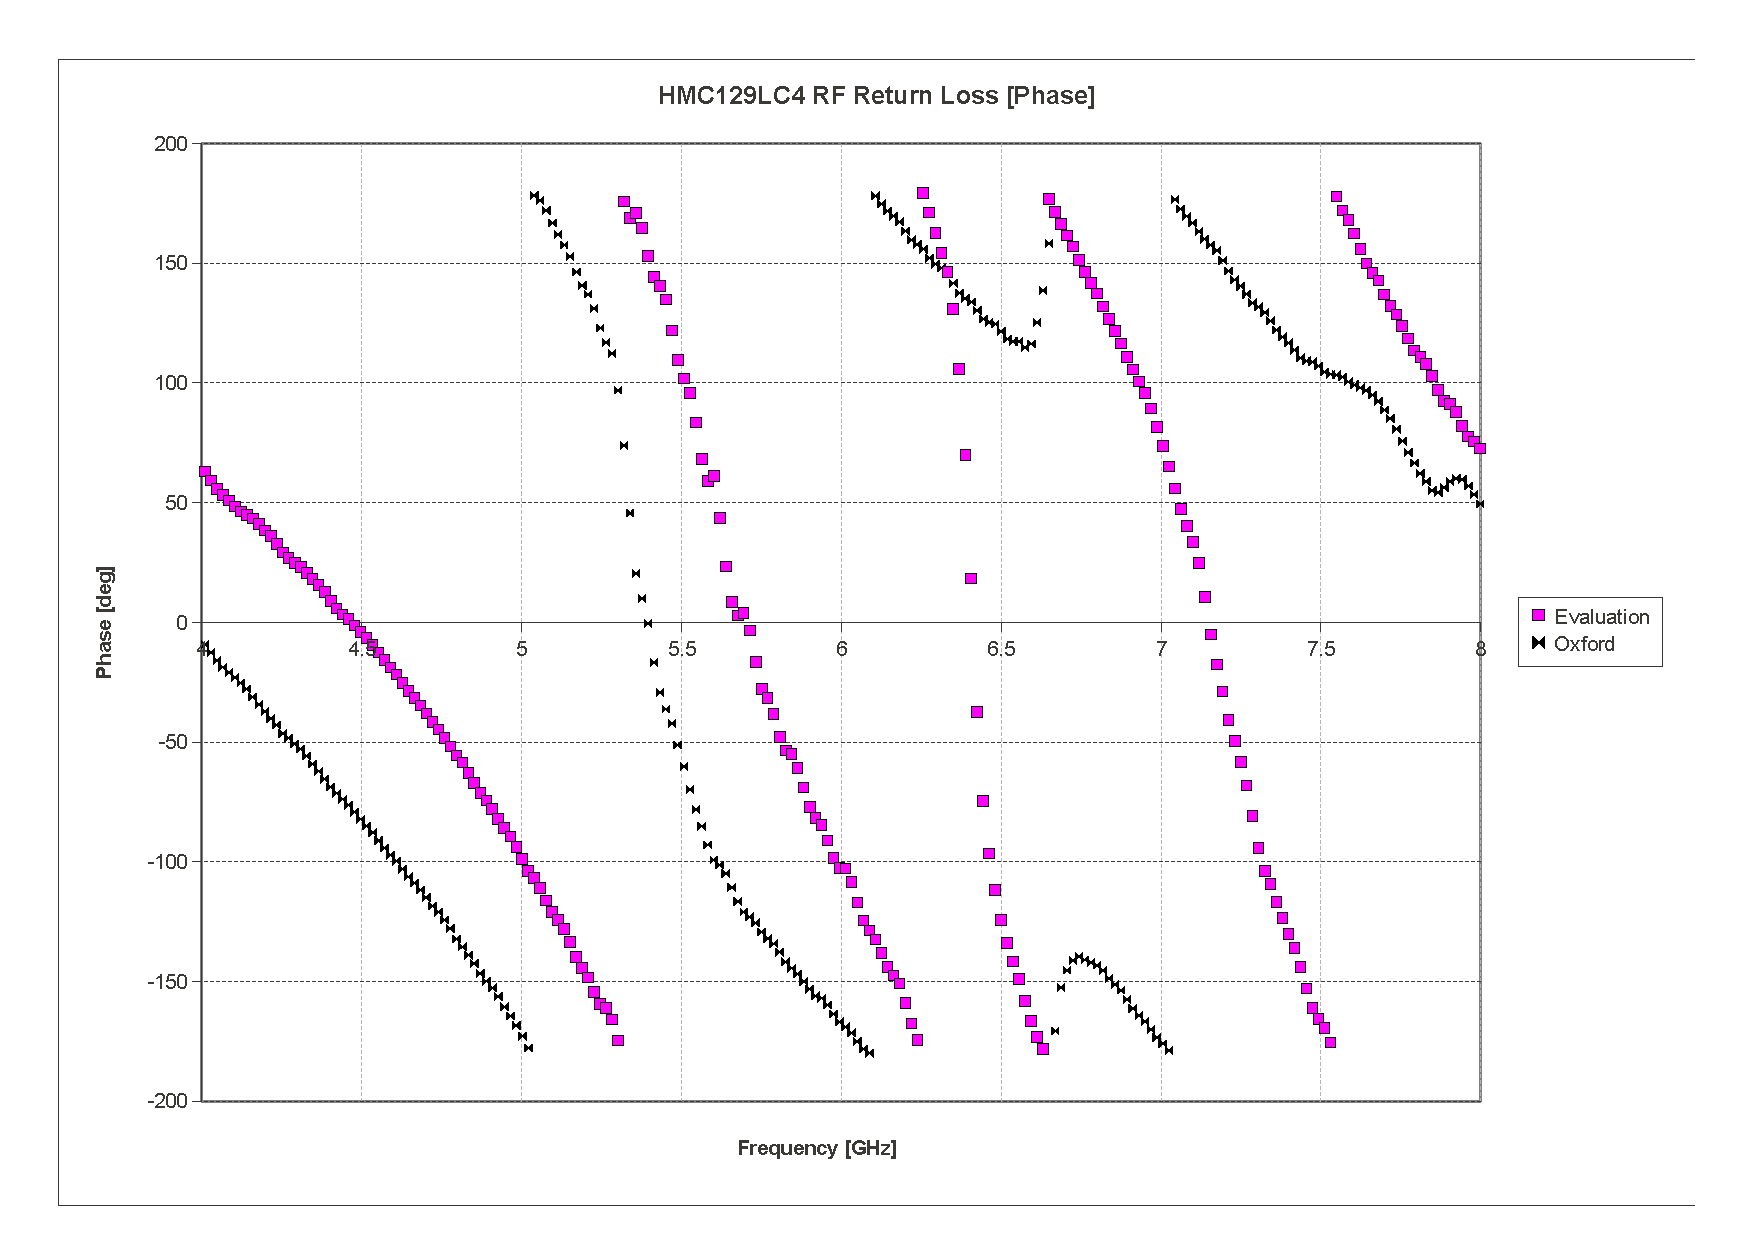
\includegraphics[height=0.45\textheight]{images/mixers/pg_0002.pdf}}
 \caption{RF Return Loss Comparison of the Hittite evaluation HMC129LC4 mixer board and the Oxford HMC129LC4 mixer board properties}
\end{figure}
\begin{figure}
\centering
\subfloat[LO Return Loss(Magnitude)]{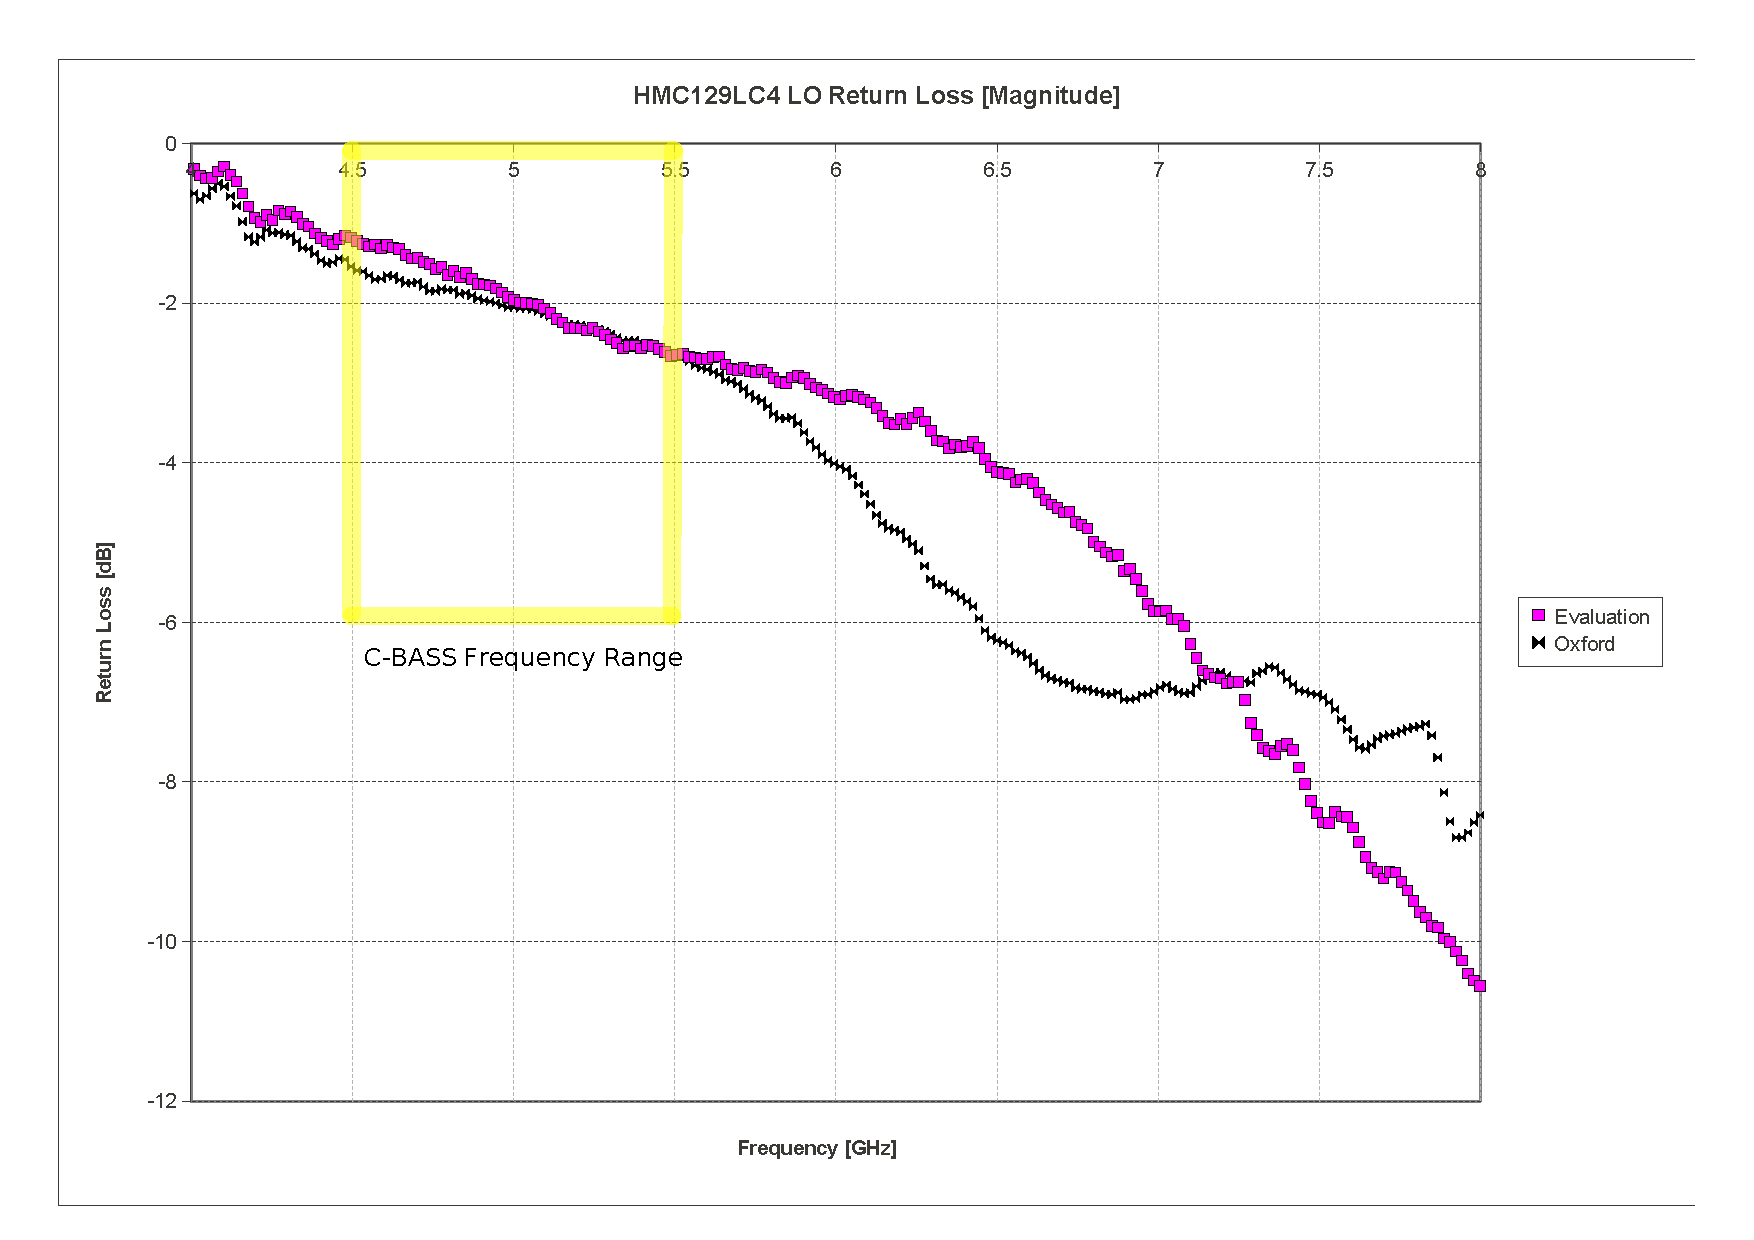
\includegraphics[width=\textwidth]{images/mixers/pg_0003a.pdf}}
\hspace{0.1cm}
%\subfloat[LO Return Loss(Phase)]{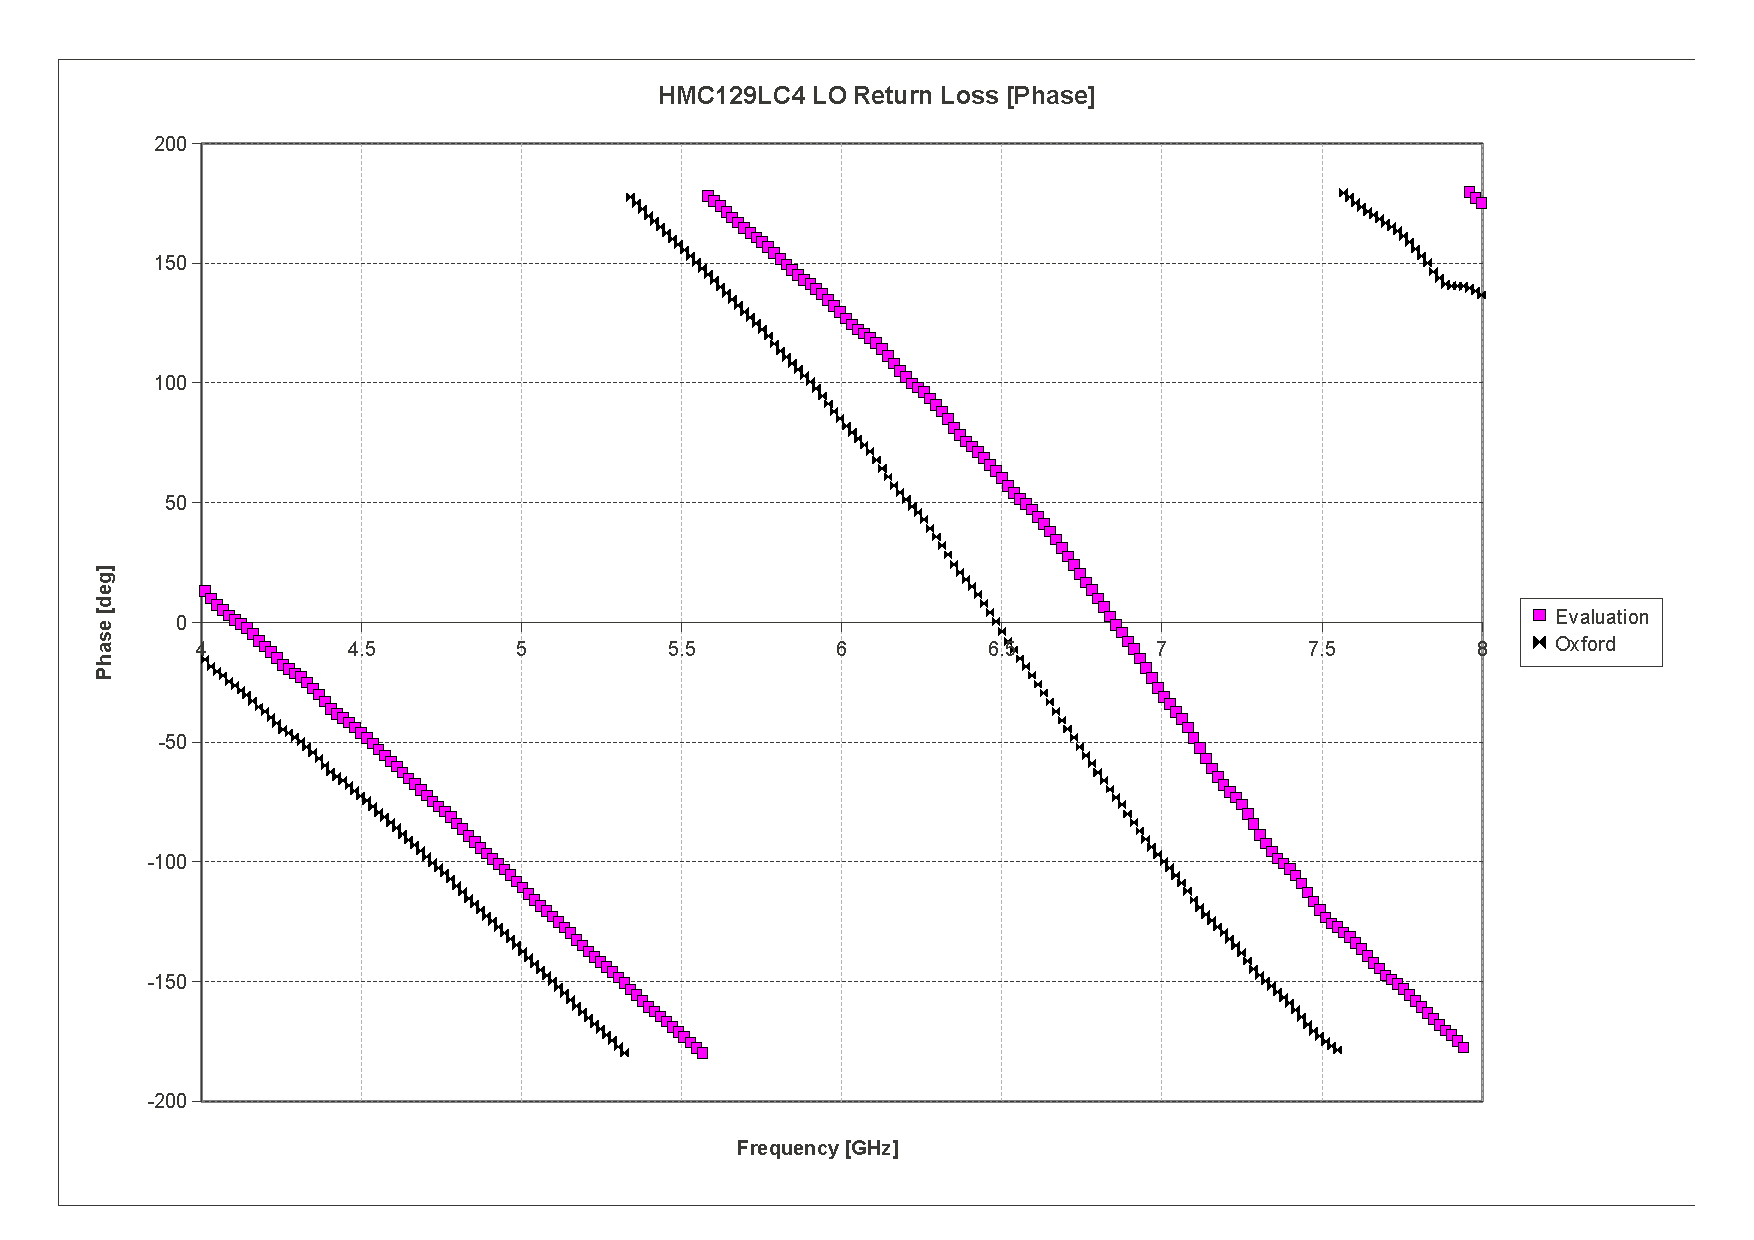
\includegraphics[height=0.45\textheight]{images/mixers/pg_0004.pdf}}
\caption{LO Return Loss Comparison of the Hittite evaluation HMC129LC4 mixer board and the Oxford HMC129LC4 mixer board properties}
\end{figure}
\begin{figure}
\centering
\subfloat[IF Return Loss(Magnitude)]{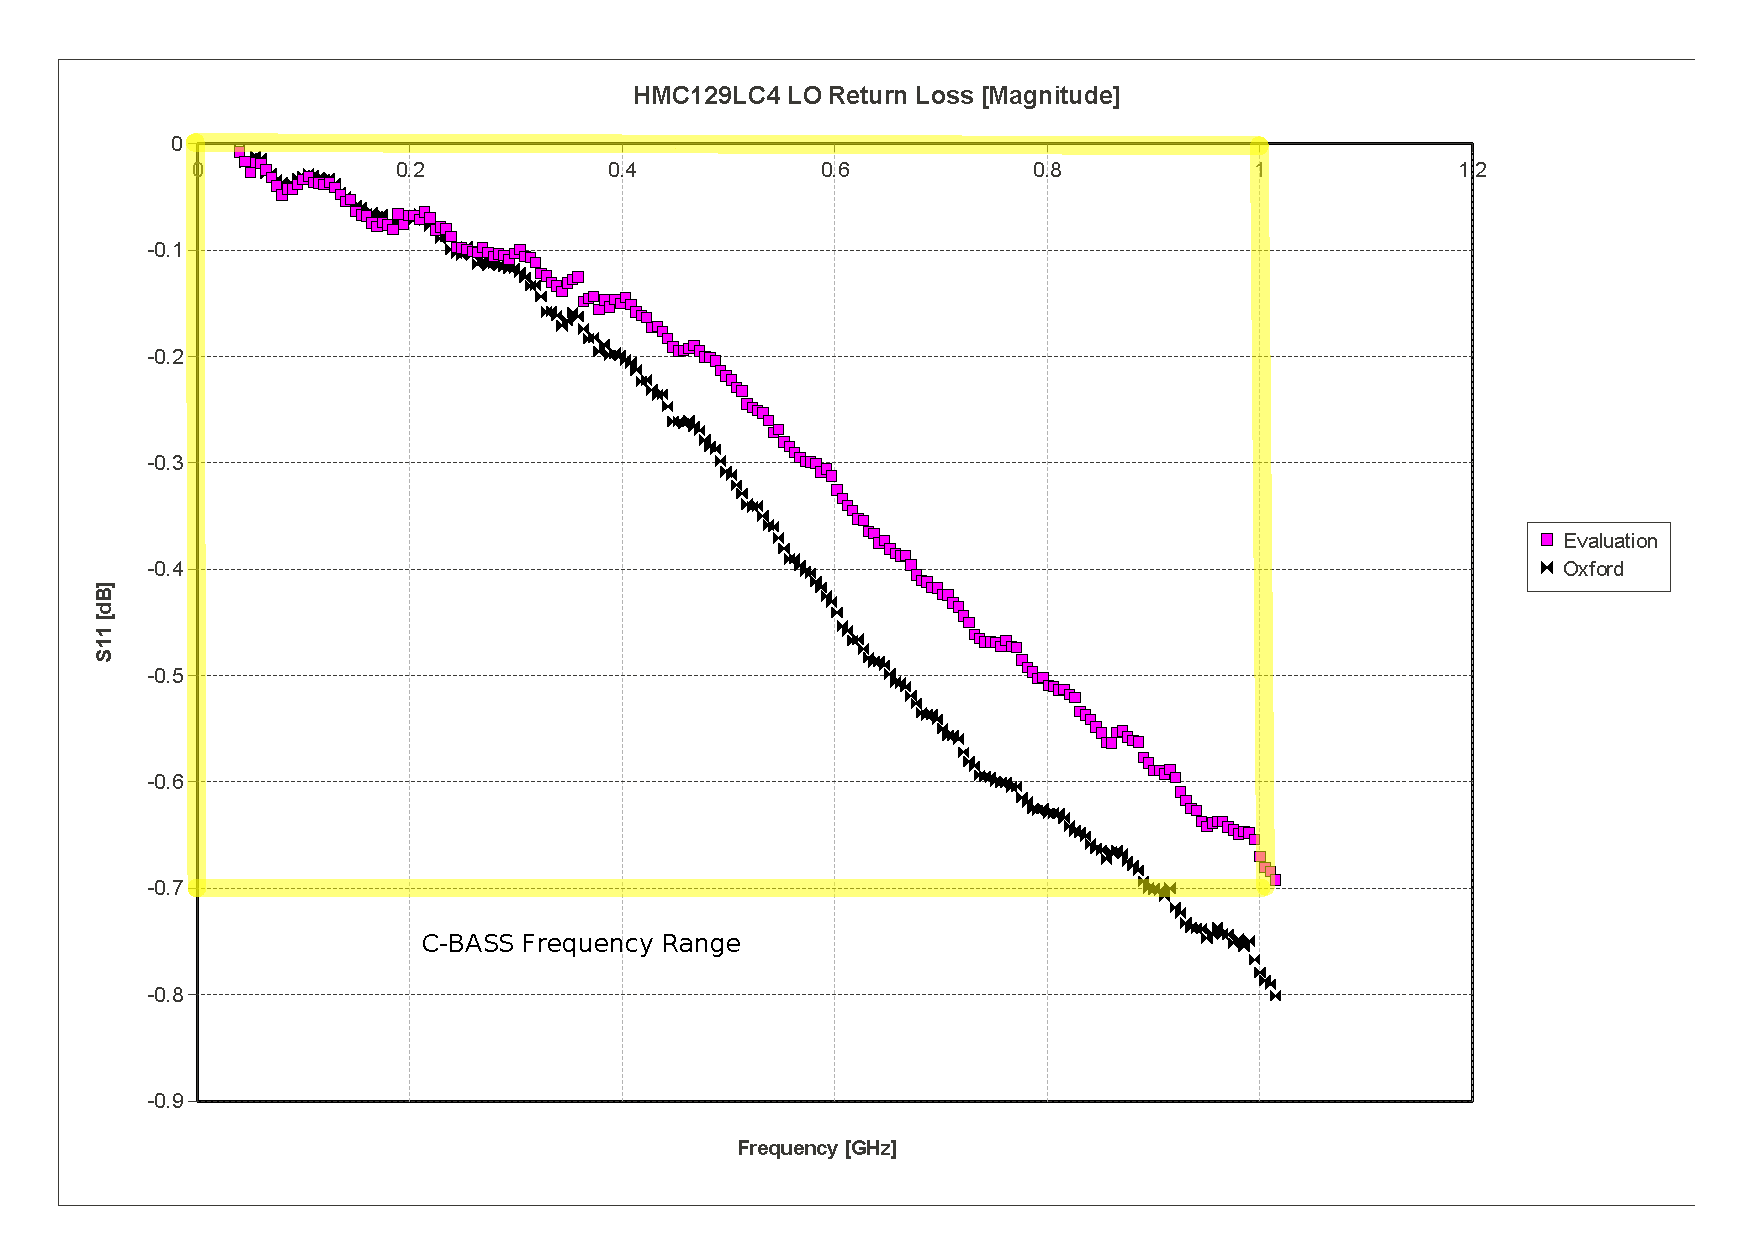
\includegraphics[width=\textwidth]{images/mixers/pg_0006a.pdf}}
\hspace{0.1cm}
%\subfloat[IF Return Loss(Phase)]{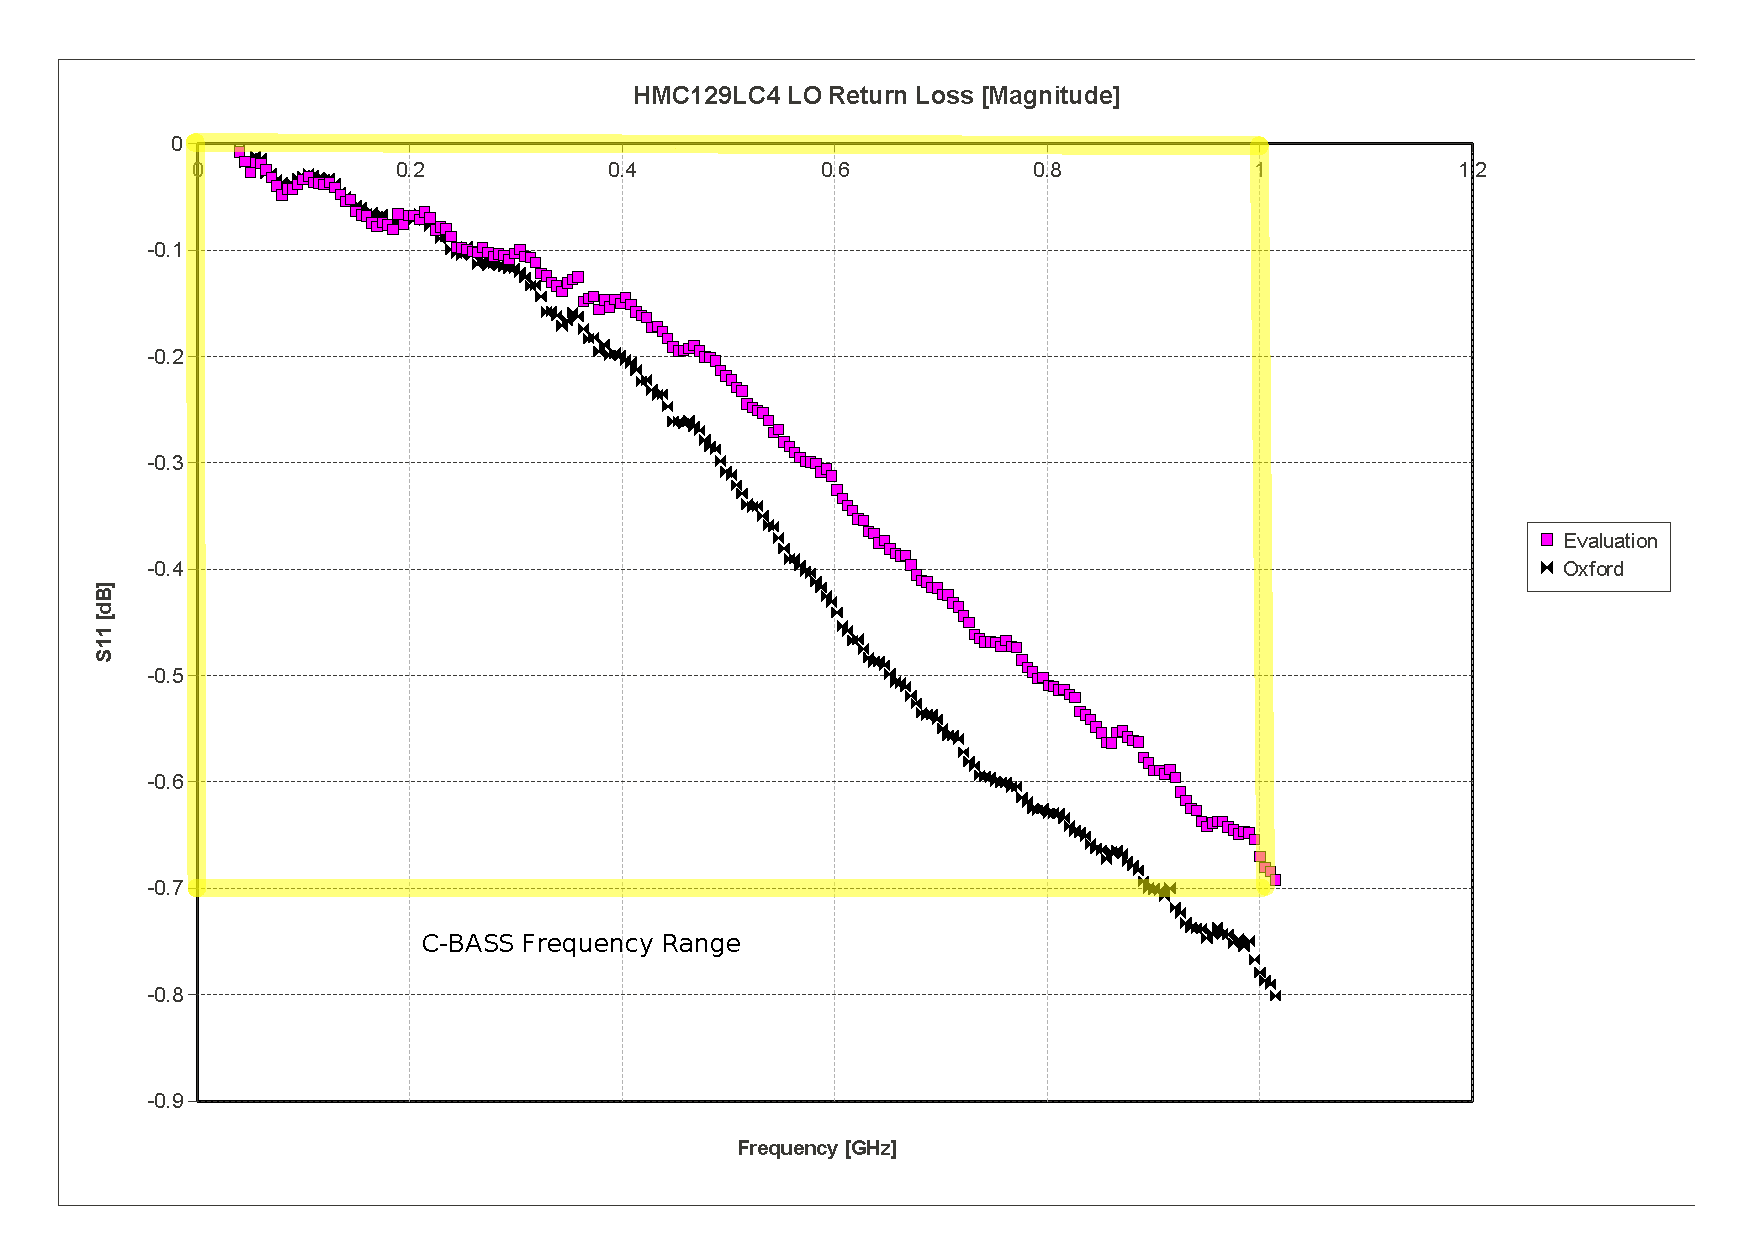
\includegraphics[width=\textwidth]{images/mixers/pg_0006.pdf}}\\

 % newdish_upgrade.jpg: 1280x728 pixel, 72dpi, 45.16x25.68 cm, bb=
 \caption{IF Return Loss Comparison of the Hittite evaluation HMC129LC4 mixer board and the Oxford HMC129LC4 mixer board properties}
% \label{fig:dish_tracking}
\end{figure}

\begin{figure}[ht]
 \centering
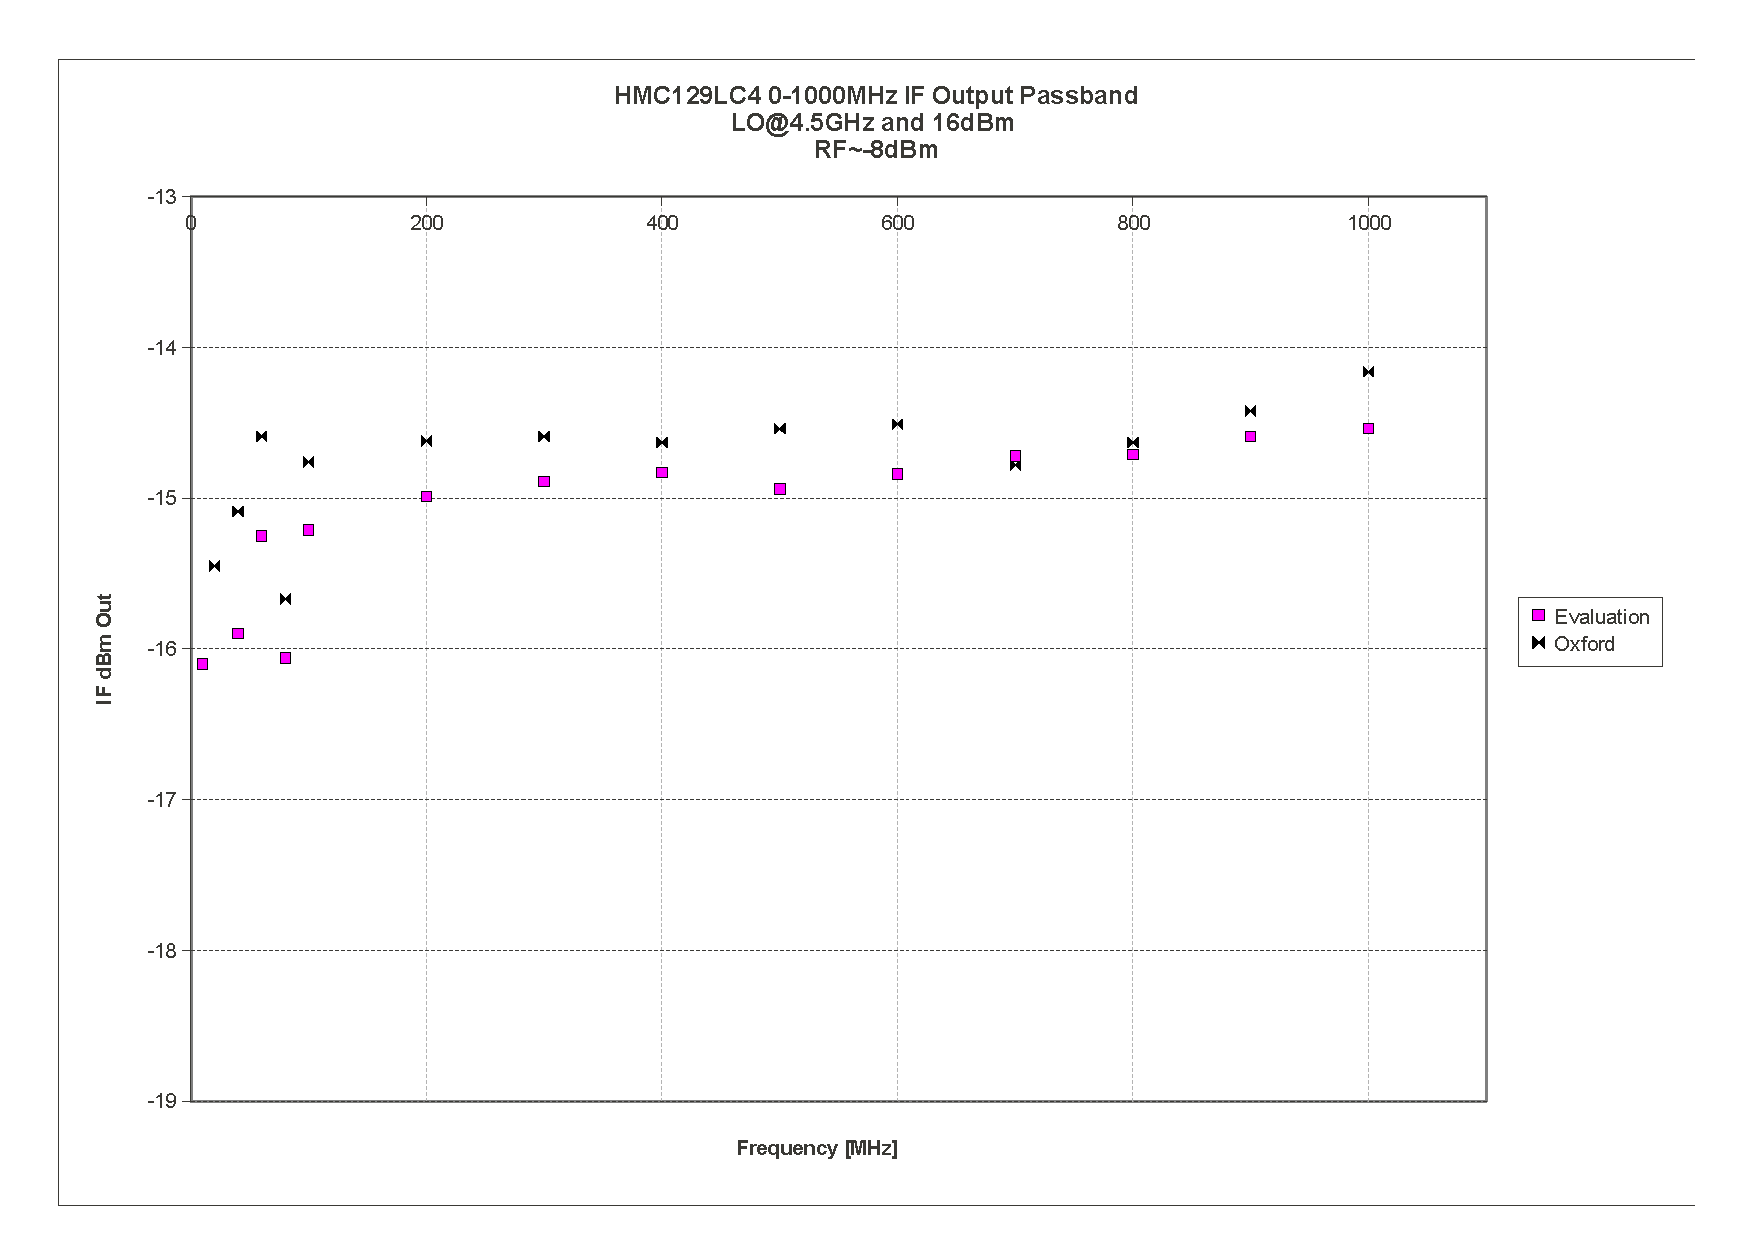
\includegraphics[height=0.5\textheight]{images/mixers/pg_0008.pdf}
 % newdish_upgrade.jpg: 1280x728 pixel, 72dpi, 45.16x25.68 cm, bb=
 \caption{Insertion loss 0$\rightarrow$1000~MHz IF band of the HMC129LC4}
% \label{fig:dish_tracking}
\end{figure}

\clearpage
\subsection{Filter Design}
\label{sec:lowfreqFilters}

For the design shown in \fign{fig:digital_receiver}, two low frequency filters are required: a 500~MHz lowpass filter and a 500$\rightarrow$1000~MHz bandpass filter.

The difficulty of designing filters in the 1GHz frequency range is that it straddles two design regions \cite{matthaei1980} . Generally higher frequency filters are designed using strip line which scale in size with wavelength making them unsuitable for use at low frequencies. Low frequency designs have tended to use lumped-element capacitors and inductors, but these are notoriously difficult to use at higher frequencies where parasitic effects become important.

The design we have employed uses a lumped-element based approach from  with ongoing development and simulations in the \textit{Microwave Office} software suite. Careful use of standardised, well understood, high quality components has allowed us to build filters at unusually high frequencies usually with rapid turnaround times. This makes use of published component values from Murata \cite{murataAWR}

Results so far are very promising. The 0$\rightarrow$500~MHz Low pass filter is complete (see Figure~\ref{fig:LowFrequency0_500MHz}) and we are rapidly converging on a suitable band-pass filter for the 500$\rightarrow$1000MHz band Figure~\ref{fig:LowFrequency500_1000MHza}. Our understanding of the behaviour of the Murata components at high frequencies has improved significantly since this version of the bandpass filter.

Component choice is an important consideration, as is symmetry in the design. We have used coplanar waveguide to allow access to the ground plane on the top side of the board, and have laid out the components in a symmetrical fashion. All components are chosen from a set of readily available Murata inductors and capacitors suitable for high frequencies with a theoretical upper limit of 2~GHz, dictated by the inductors self resonant frequencies. As can be seen in \fign{fig:filterBoxing}, careful consideration also needs to be given to the way in which the filter boards are packaged. The packaging plays an important role in improving the out of band rejection characteristics.

\begin{figure}
 \centering
 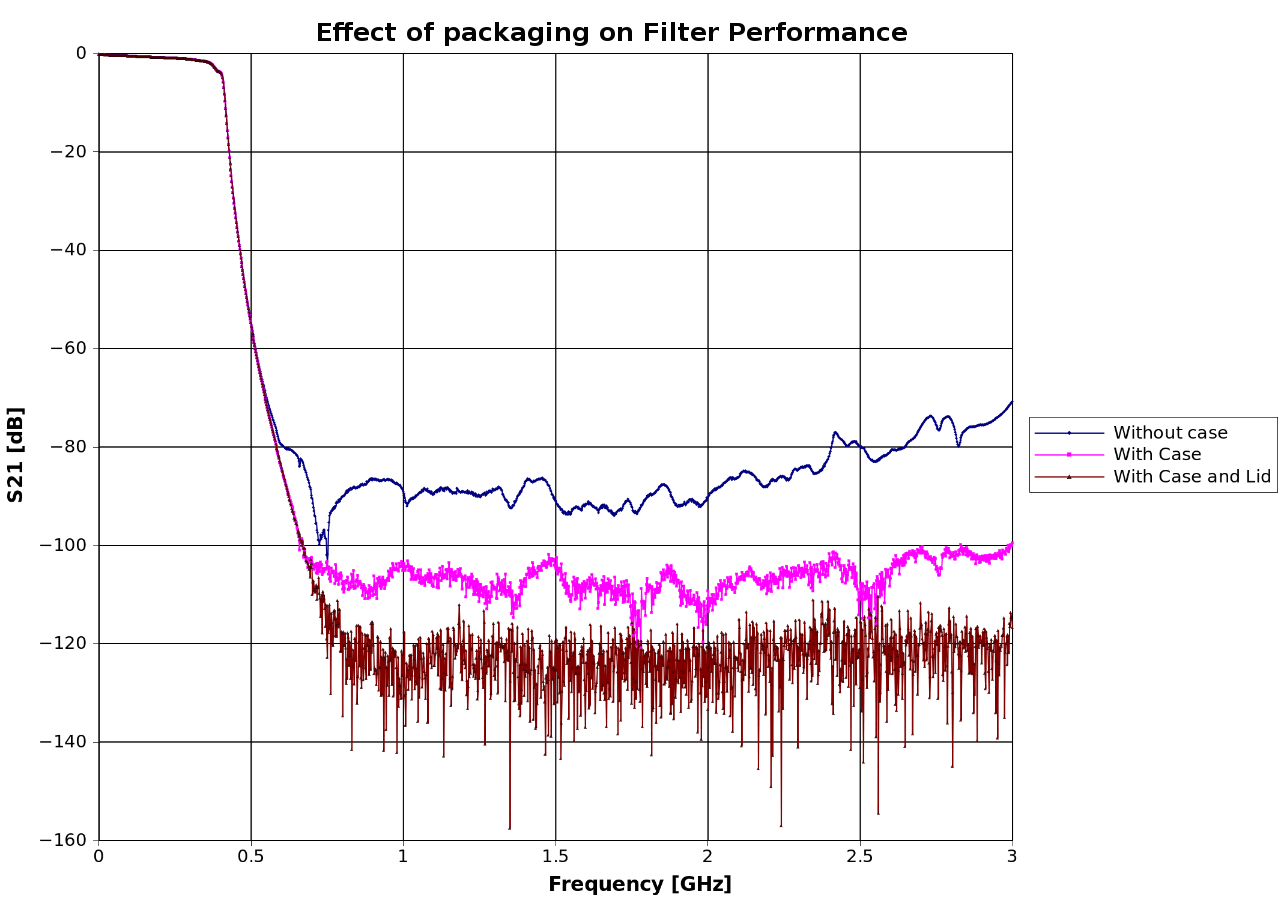
\includegraphics[width=\textwidth]{./images/LowFrequencyFilters/filterBoxing.png}
 % filterBoxing.png: 1319x930 pixel, 72dpi, 46.53x32.80 cm, bb=0 0 1319 930
 \caption{Comparison of different stages of the Filter construction process. These plots show the importance of properly enclosing the filter boards}
 \label{fig:filterBoxing}
\end{figure}


\begin{figure}
 \centering
\subfloat[][Lowpass filter design schematic]{
 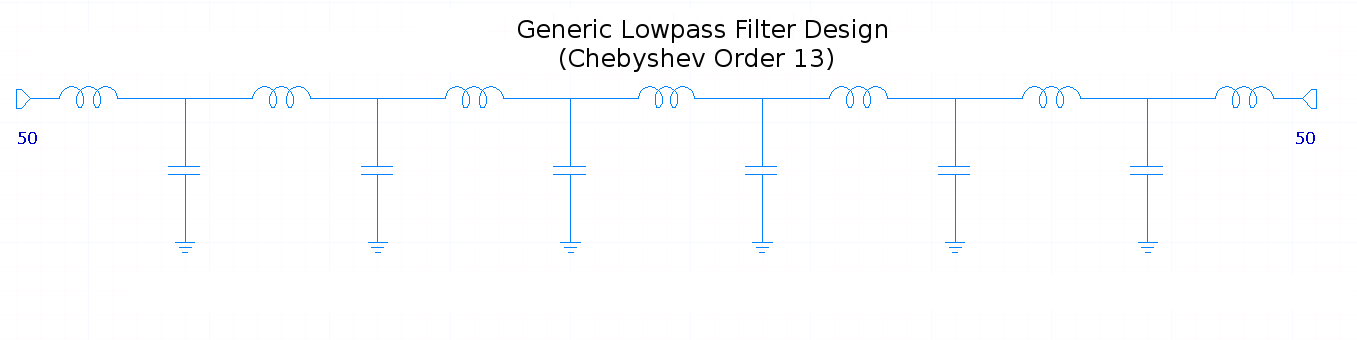
\includegraphics[width=\textwidth]{./images/LowFrequencyFilters/lowpass.png}
}\\
\subfloat[][Bandpass filter design schematic]{
 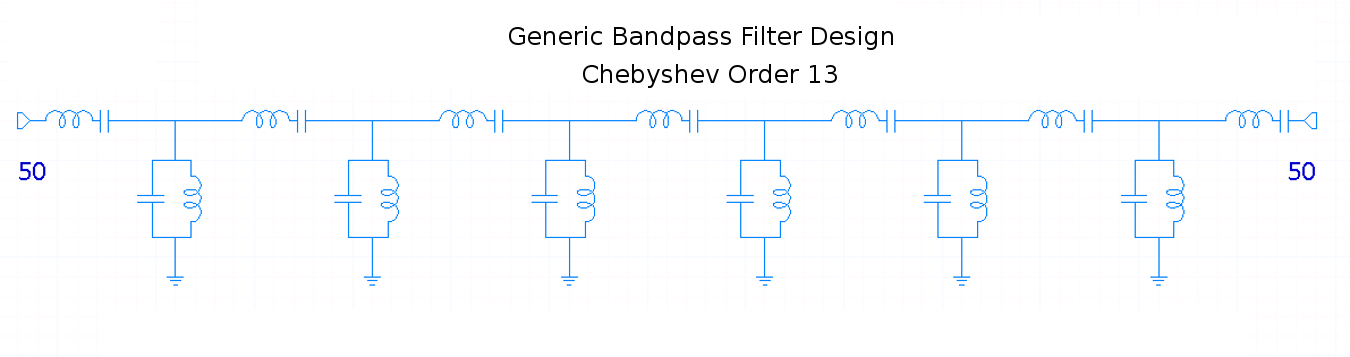
\includegraphics[width=\textwidth]{./images/LowFrequencyFilters/bandpass.png}
}\\
\subfloat[][Final low frequency filter built into compact box. Notice the symmetry in the placement of components. The complete filter features a copper lid soldered into place completely sealing the unit. We have found that the boxing and lids are very important for optimal filter performance, as is apparent from \fign{fig:filterBoxing}. Also notice the solder joint between the PCB and the box wall. This reduces high frequency resonance artifacts, presumably caused by the exposed (otherwise) exposed cavity]{
 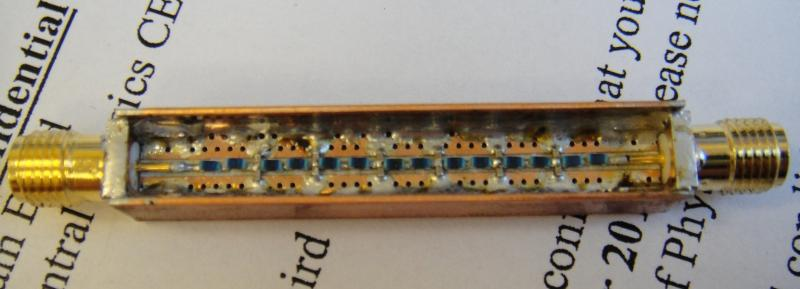
\includegraphics[width=\textwidth]{./images/LowFrequencyFilters/DSC03823a.jpg}
}

 % lowpass.png: 1357x340 pixel, 72dpi, 47.87x11.99 cm, bb=0 0 1357 340
 \caption{Low frequency lumped element filter designs and manufacture}
 \label{fig:filterDesigns}
\end{figure}


\begin{figure}
 \centering
\subfloat[][]{
 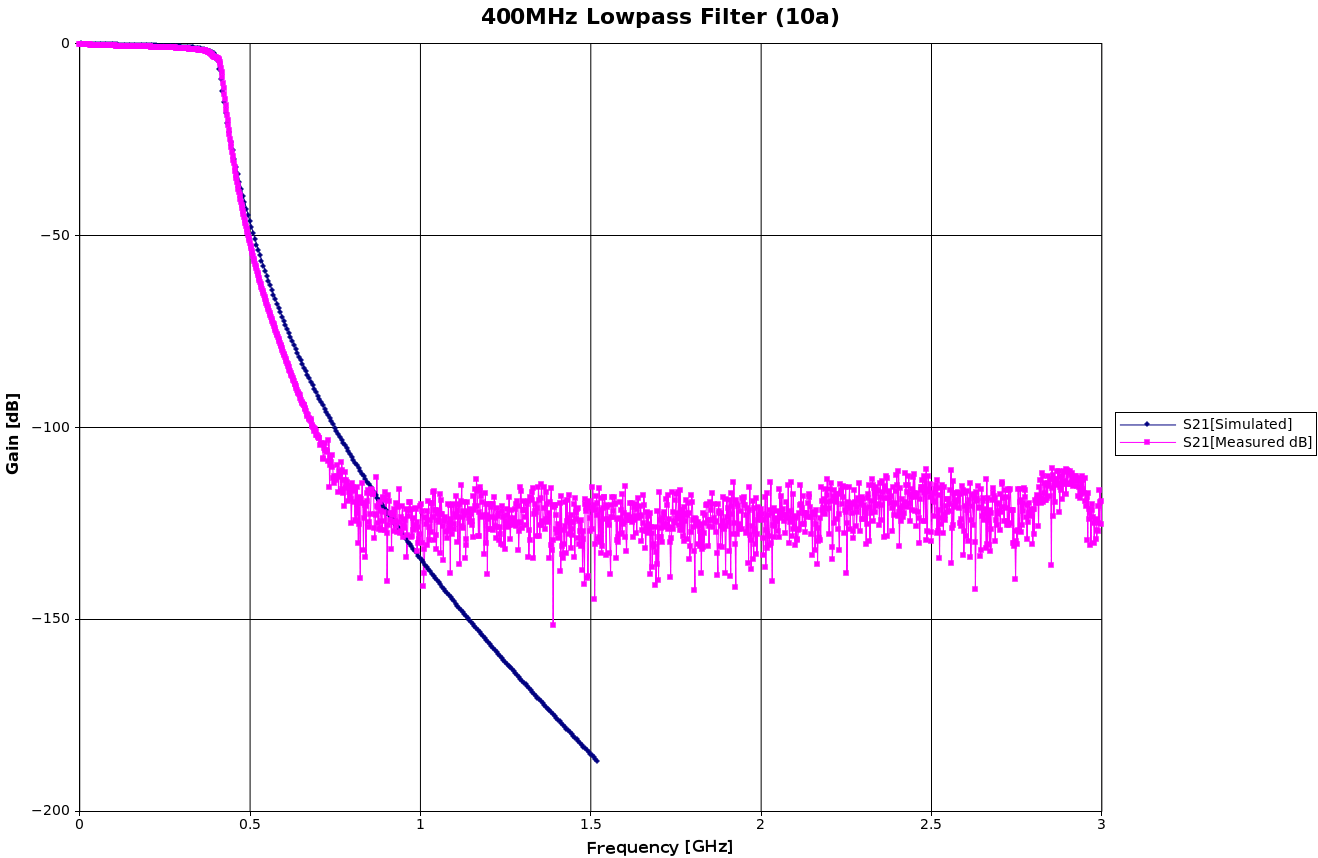
\includegraphics[height=0.4\textheight]{./images/LowFrequencyFilters/lpf10asimvsmeasured1.png}
}\\
\subfloat[][]{
 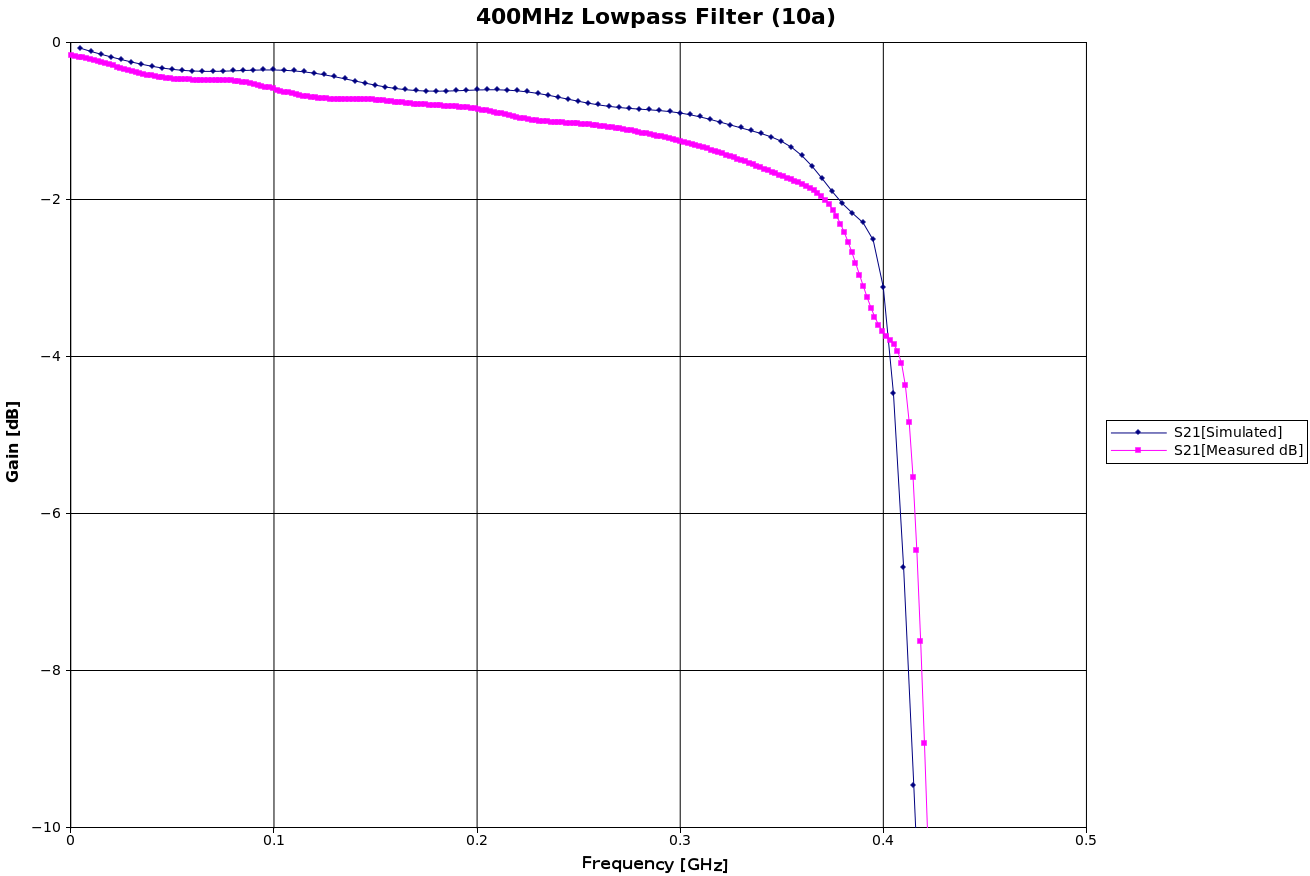
\includegraphics[height=0.4\textheight]{./images/LowFrequencyFilters/lpf10asimvsmeasured2.png}
}
 % lpf10asimvsmeasured1.png: 1571x1046 pixel, 72dpi, 55.41x36.90 cm, bb=0 0 1571 1046
 \caption{Simulated filter performance against measured performance. }
 \label{fig:simvsmeasuredlpf10a}
\end{figure}


We focused on using a design/manufacture technique that would allow rapid prototyping of these filters, and allow quick turnaround times for custom filters that might be required in the future. The techniques we have developed allow a custom filter built in a day, with the major bottleneck still being availability of components. This allows significantly more flexible designs to be produced than was the case previously. In addition, the technique opens up the possibility of building compact filters directly onto printed circuit boards using pick and place for mass production. This has potential for use in large scale radio astronomy deployments such as the Square Kilometer Array. 

% \begin{figure}
%  \centering
%  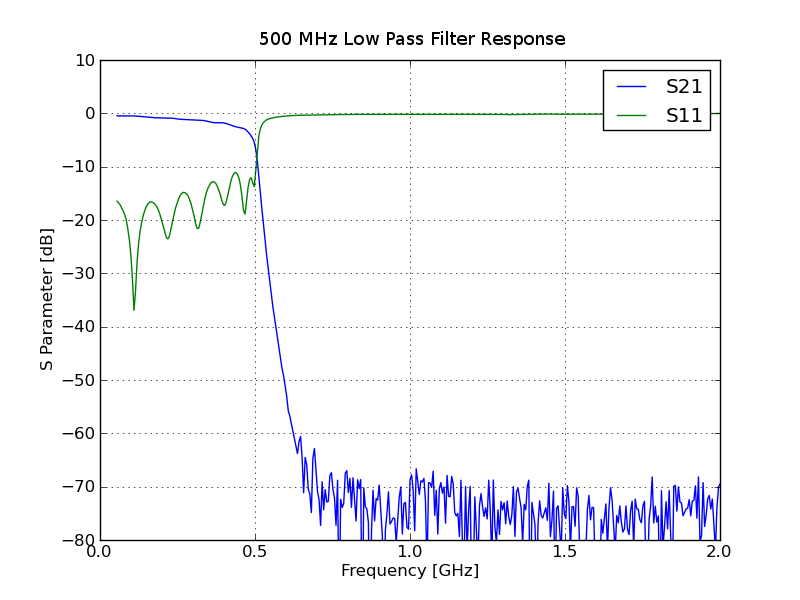
\includegraphics[width=0.5\textwidth]{./images/LowFrequencyFilters/LPF1.png}
%  \caption{The 0$\rightarrow$500MHz Low pass filter. }
%  \label{fig:LowFrequency0_500MHz}
% \end{figure}


 
\begin{figure}
 \centering
\subfloat[The 0$\rightarrow$500MHz Low pass filter.]{
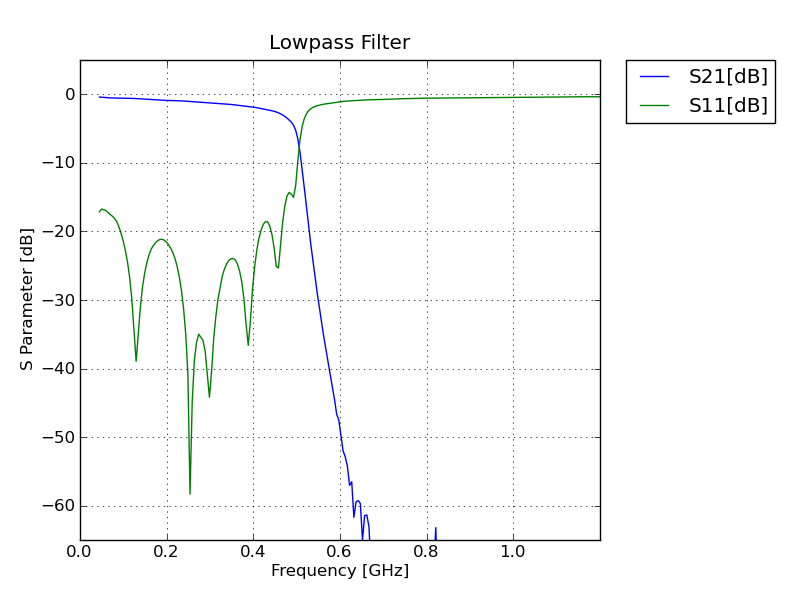
\includegraphics[width=0.5\textwidth]{./images/LowFrequencyFilters/LowpassFilter.png}
\label{fig:LowFrequency0_500MHz}
}\\
\subfloat[The 1000~MHz low pass filter ]{
 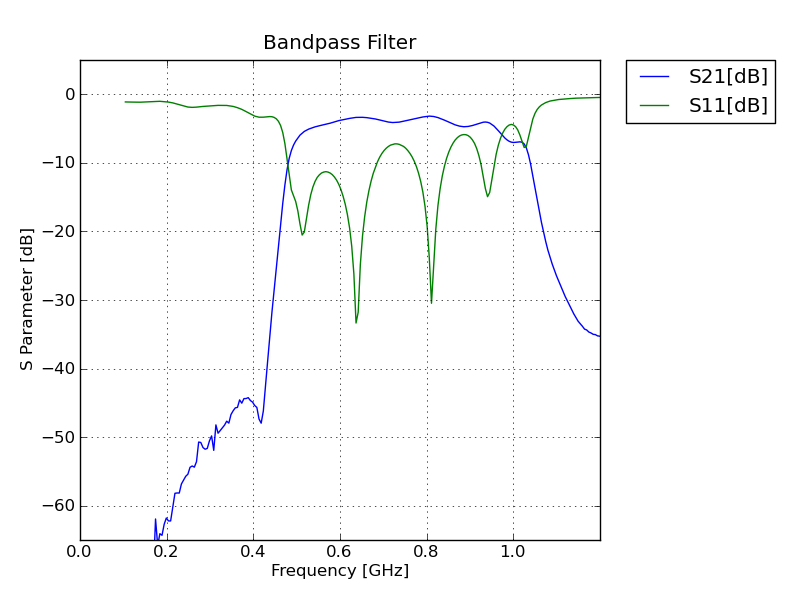
\includegraphics[width=0.5\textwidth]{./images/LowFrequencyFilters/BandpassFilter}
\label{fig:LowFrequency500_1000MHza}}
\label{fig:LowFrequencyFilters} 
\caption{The 500~MHz lowpass filter and the 500$\rightarrow$1000MHz bandpass filter. Since the bandpass filter operates at high frequenciess where lumped element design is difficult, we decided to make the band pass filter from a cascaded high pass filter (500MHz) and low pass filter (1000MHz). This allowed us to optimise the high end and low end independently. There is still a little work to do on the 1000~MHz filter (i.e the high end of the bandpass filter), but out understanding of these components' behavious at high frequency has improved significantly, and we believe this will be reflected in the next iteration}
\end{figure}